% Copyright 2005-2016 Airbus-EDF-IMACS-Phimeca
% Permission is granted to copy, distribute and/or modify this document
% under the terms of the GNU Free Documentation License, Version 1.2
% or any later version published by the Free Software Foundation;
% with no Invariant Sections, no Front-Cover Texts, and no Back-Cover
% Texts.  A copy of the license is included in the section entitled "GNU
% Free Documentation License".
\renewcommand{\filename}{docUC_StocProc_DensitySpectralFunction_UserDefined.tex}
\renewcommand{\filetitle}{UC : Creation of a User defined spectral density function}

% \HeaderNNIILevel
% \HeaderIILevel
\HeaderIIILevel

\label{SpectralModelCreation}
\index{Stochastic Process!Spectral Model}

Let $X: \Omega \times \cD \rightarrow \Rset^d$  be a multivariate  stationary normal process of dimension $d$. We only treat here the case where the domain is of dimension 1: $\cD \in \Rset$ ($n=1$). \\
If the process is continuous, then $\cD=\Rset$. In the discrete case, $\cD$  is a lattice. \\


$X$ is supposed to be a second order process with zero mean and we suppose that its spectral density function $S : \Rset \rightarrow \mathcal{H}^+(d)$ defined in (\ref{specdensFunc}) exists. $\mathcal{H}^+(d) \in \mathcal{M}_d(\Cset)$ is the set of $d$-dimensional positive definite hermitian matrices.\\

This use case illustrates how the User can define his own density spectral function from parametric models. OpenTURNS allows it   thanks to the object {\itshape UserDefinedSpectralModel} defined from :
\begin{itemize}
\item a frequency grid $(-f_c, \dots, f_c)$ with step  $\delta f$, stored in the object \emph{RegularGrid},
\item a collection of hermitian matrices $\in \mathbb{M}_d(\mathbb{C})$ stored in the object \emph{HermitianMatrixCollection}, which are the images of each point of the frequency grid through the density spectral function.
\end{itemize}

OpenTURNS builds a constant piecewise function on  $[-f_c,f_c]$, where the intervals where the density spectral function is constant are centered on the points of the frequency grid, of length $ \delta f$. Then, it is  possible to evaluate the spectral density function for a given frequency thanks to the method {\itshape computeSpectralDensity}: if the frequency is not inside the interval  $[-f_c,f_c]$, OpenTURNS returns an exception. Otherwise, it returns the hermitian matrix of the subinterval of $[-f_c,f_c]$ that contains the given frequency.\\


\requirements{

  \begin{description}
  \item[$\bullet$] a frequency grid : {\itshape myFrequencyGrid}
  \item[type:]  RegularGrid
  \end{description}

  \begin{description}
  \item[$\bullet$] a collection of hermitian matrices : {\itshape myHermitianCollection}
  \item[type:]  HermitianMatrixCollection
  \end{description}

}
{
  \begin{description}
  \item[$\bullet$] a spectral model : {\itshape mySpectralModel}
  \item[type:] SpectralModel
  \end{description}

}

\textspace\\
Python script for this UseCase :

\inputscript{script_docUC_StocProc_DensitySpectralFunction_UserDefined}

\textspace\\

In the following example, we illustrate how to create a modified low pass model of dimension $d=1$ with exponential decrease defined by : $S : \mathbb{R} \rightarrow  \mathbb{R} $ where
\begin{itemize}
\item Frequency value $f$ should be positive,
\item for $f < 5 Hz$, the spectral density function is constant : $S(f)=1.0$,
\item for $f > 5 Hz$, the spectral density function is equal to $S(f) = \exp \left[- 2.0 (f - 5.0)^2 \right]$.
\end{itemize}
The frequency grid is $]0, f_c] = ]0,10]$ with $\delta f = 0.2$ Hz. The Figure \ref{UserDefinedSpectralModelDemonstration} draws the  spectral density.

        \begin{figure}[H]
          \begin{center}
            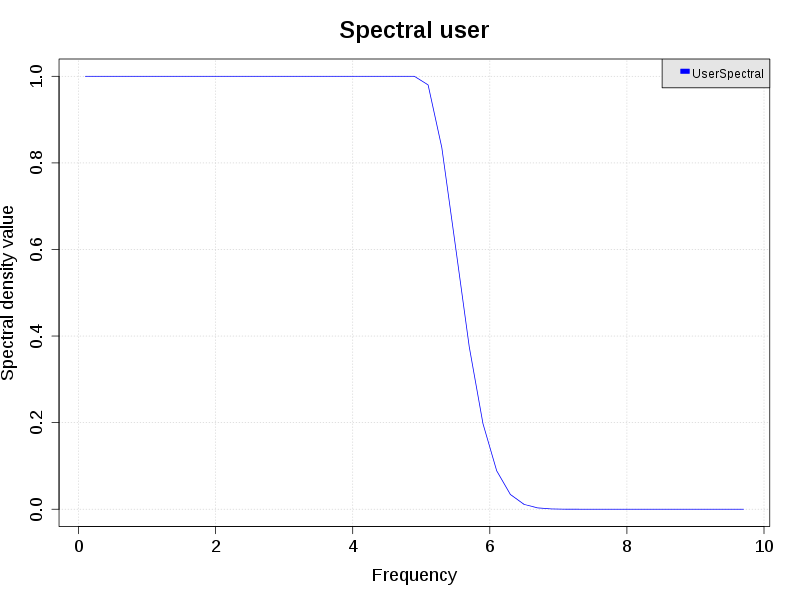
\includegraphics[width=7cm]{Figures/UserDefinedSpectralModelDemonstration.png}
            \caption{User defined spectral model}
            \label{UserDefinedSpectralModelDemonstration}
          \end{center}
        \end{figure}
